%!TEX root = ../thesis.tex

\section{Algorithm explaination}\label{section:algorithm}

The polynomial-time algorithm introduced in \cite{PPPptime2016} describes a recursive procedure for reducing a red-black graph to an empty graph, if it admits a persistent phylogeny.
The recursion stops either when the base case is reached - empty graph (line \ref{algorithm:reduce:ifempty}) - or when the algorithm can't compute a successful c-reduction for \grb{} - the graph reaches a state of irreducibility (line \ref{algorithm:reduce:ifnosource}).

The procedure for a Reduce function is given below.

\begin{algorithm}[h]
  \caption{Reduce. Recursive reduction of a red-black graph.}\label{algorithm:reduce}

  \SetKwData{Source}{\ensuremath{s}}
  \SetKwData{Sc}{\ensuremath{S_{c}}}
  \SetKwInOut{Input}{Input}
  \SetKwInOut{Output}{Output}

  \Input{Red-black graph \grb{}}
  \Output{c-reduction of the graph \grb{}, if it exists}

  \BlankLine

  Remove singletons from \grb{}\;\label{algorithm:reduce:rmsingle}

  \If{\grb{} is empty}{\label{algorithm:reduce:ifempty}
    \Return $\langle$ $\rangle$\;
  }

  \BlankLine

  \If{\grb{} has a free character \character{}}{\label{algorithm:reduce:iffree}
    \grb{} $\gets$ Realize(\character[][-], \grb{})\;

    \Return $\langle$ \character[][-], Reduce(\grb{}) $\rangle$\;
  }

  \BlankLine

  \If{\grb{} has a universal character \character{}}{\label{algorithm:reduce:ifuniversal}
    \grb{} $\gets$ Realize(\character[][+], \grb{})\;

    \Return $\langle$ \character[][+], Reduce(\grb{}) $\rangle$\;
  }

  \BlankLine

  \If{\grb{} has k > 1 connected components}{\label{algorithm:reduce:ifdisconnected}
    \Return $\langle$ Reduce($\grb{}_{0}$), \dots, Reduce($\grb{}_{k-1}$) $\rangle$\;
  }

  \BlankLine

  \gm{} $\gets$ maximal reducible graph of \grb{}\;

  \hasse{} $\gets$ Hasse diagram for \gm{}\;

  \BlankLine

  \If{\hasse{} has no safe source}{\label{algorithm:reduce:ifnosource}
    Abort\;
  }

  \BlankLine

  \Source $\gets$ Find-initial-state(\hasse{})\;

  \Sc $\gets$ sequence of positive characters of \Source that are inactive in \grb{}\;

  \grb{} $\gets$ Realize(\Sc, \grb{})\;

  \BlankLine

  \Return $\langle$ \Sc, Reduce(\grb{}) $\rangle$\;
\end{algorithm}

The Reduce procedure computes signed character realizations with the support of a Realize function, which follows the definition of Realization (\ref{definition:realization}) and extends it to support a list of signed characters as input.

We will address the Find-initial-state procedure in detail in section \ref{section:safe-chains-sources}.

\subsection{Preparing the graph}\label{section:preparing-the-graph}

An explaination of lines \ref{algorithm:reduce:rmsingle} to \ref{algorithm:reduce:ifdisconnected} has already been provided in section \ref{section:grb}.

The first steps of the Reduce procedure (algorithm \ref{algorithm:reduce}) serve the purpose of bringing the red-black graph to a state which can't be "pruned" further.
Removing isolated vertices (singletons), realizing free and universal characters, and reducing each connected component of \grb{} separately is all part of preparing the graph for a more thorough analysis.

\subsection{Maximal reducible graph and Hasse diagram}\label{section:gm-hassediagram}

Let us introduce the concept of \emph{maximal} character. A character \character{} is maximal in a red-black graph \grb{} if $S(\character{}) \not\subset S(\character[i])$ for each inactive character \character[i] of \grb{}. Two maximal characters \character[0] and \character[1] can overlap, i.e., share common species, but clearly they can't be included in one another. Moreover, to clarify what we just described, we say that a character \character[0] includes another character \character[1] if $S(\character[0]) \supseteq S(\character[1])$.

The set of maximal characters of \grb{} is then used to build a maximal reducible graph \grbcm{} from it.

\begin{definition}[Maximal reducible graph]\label{definition:maximal-reducible-graph}
  Let \grb{} be a red-black graph and \cm{} its set of maximal characters.

  The maximal reducible graph \grbcm{}, \gm{} for short, is the red-black graph induced in \grb{} by the set \cm{} of characters.

  \gm{} consists of the subgraph of \grb{} that has the characters in \cm{} and the species of \grb{} adjacent to \cm{}.
\end{definition}

To be able to compute a successful c-reduction for a graph \grb{} we need to represent the set of species of its maximal reducible graph \gm{} as a Hasse diagram \cite{PPPptime2016}.
The Hasse diagram is used to represent partially ordered sets (poset), defined as $(P_{s}, \leq)$, where each element of $P_{s}$ is a vertex in the diagram and there exists an edge from a vertex $a$ to $b$ if and only if $a < b$ and there doesn't exist a vertex $c$ such that $a < c < b$.

The definition of Hasse diagram translates in our algorithm as a directed acyclic graph, where the vertices of $P_{s}$ are made up of the species of \gm{}.

\begin{definition}[Hasse diagram for \grbcm{}]\label{definition:hasse-diagram}
  Let \gm{} be a maximal reducible graph.

  The Hasse diagram \hasse{} for \gm{} is the Hasse diagram for the poset $(P_{s}, \leq)$ of the species of \gm{} ordered by the relation $\leq$.
  Two species \species[1] and \species[2] of $P_{s}$ are in a relation $\species[1] \leq \species[2]$ if $C(\species[1]) \subseteq C(\species[2])$
\end{definition}

Each vertex of a Hasse diagram \hasse{} consists of a set of species which share the same characters, while each edge \edge{v_{i}}{v_{i+1}} of the diagram is labeled by the set of positive characters that are in $v_{i+1}$ and not in $v_{i}$. When a character \character{} "is in" a vertex $v_{i}$, it means that all the species that label $v_{i}$ have the character \character{} in their set $C(\species{})$.

We show an example of maximal reducible graph and its corresponding Hasse diagram.

\begin{figure}[h]
  %!TEX root = ../thesis.tex

\centering
  \begin{subfigure}[b]{0.98\textwidth}
    \centering
      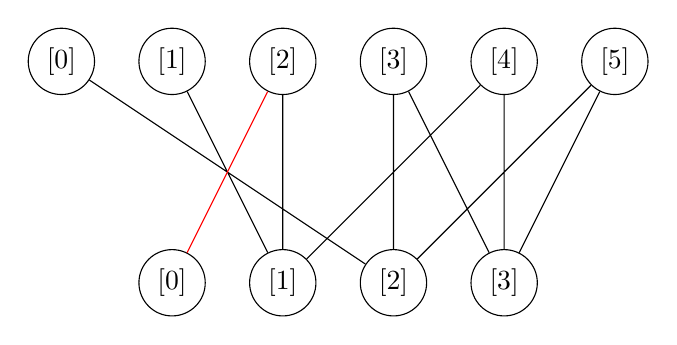
\begin{tikzpicture}
        {\tikzstyle{every node}=[circle, draw]
          \foreach \i in {0, ..., 5}
          {
            \node (s\i) at (\i*40pt, 80pt) {\species[\i]};
          }

          \foreach \j in {0, ..., 3}
          {
            \node (c\j) at (\j*40pt+40pt, 0) {\character[\j]};
          }
        }

        \draw
          (c3) -- (s3)
          (c3) -- (s4)
          (c3) -- (s5)
          (c1) -- (s1)
          (c1) -- (s2)
          (c1) -- (s4)
          (c2) -- (s0)
          (c2) -- (s3)
          (c2) -- (s5);

        \draw[red]
          (c0) -- (s2);
      \end{tikzpicture}

    \caption{Maximal reducible graph \gm{}}
    \label{figure:4:a}
  \end{subfigure}

  \bigskip

  \begin{subfigure}[b]{0.98\textwidth}
    \centering
      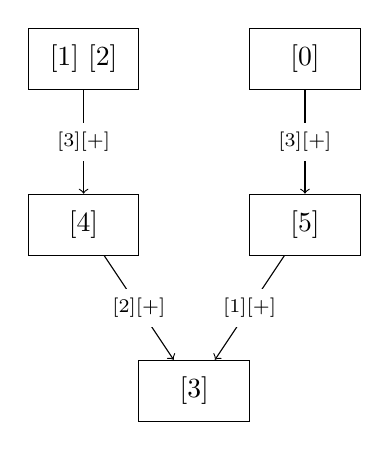
\begin{tikzpicture}
        {\tikzstyle{every node}=[rectangle, draw, minimum width=40pt, minimum height=22pt]
          \node (s1) at (0pt,  120pt) {\species[1] \species[2]};
          \node (s0) at (80pt, 120pt) {\species[0]};
          \node (s4) at (0pt,   60pt) {\species[4]};
          \node (s5) at (80pt,  60pt) {\species[5]};
          \node (s3) at (40pt,   0pt) {\species[3]};
        }

        {\tikzstyle{every node}=[fill=white, font=\scriptsize]
          \draw
            (s0) edge[->] node{\character[3][+]} (s5)
            (s1) edge[->] node{\character[3][+]} (s4)
            (s4) edge[->] node{\character[2][+]} (s3)
            (s5) edge[->] node{\character[1][+]} (s3);
        }
      \end{tikzpicture}

    \caption{Hasse diagram \hasse{} for \gm{}}
    \label{figure:4:b}
  \end{subfigure}


  \caption{Graph \gm{} and its Hasse diagram \hasse{}}\label{figure:4}
\end{figure}

\subsection{Safe chains and sources}\label{section:safe-chains-sources}
